\begin{figure}[t]
\centering
 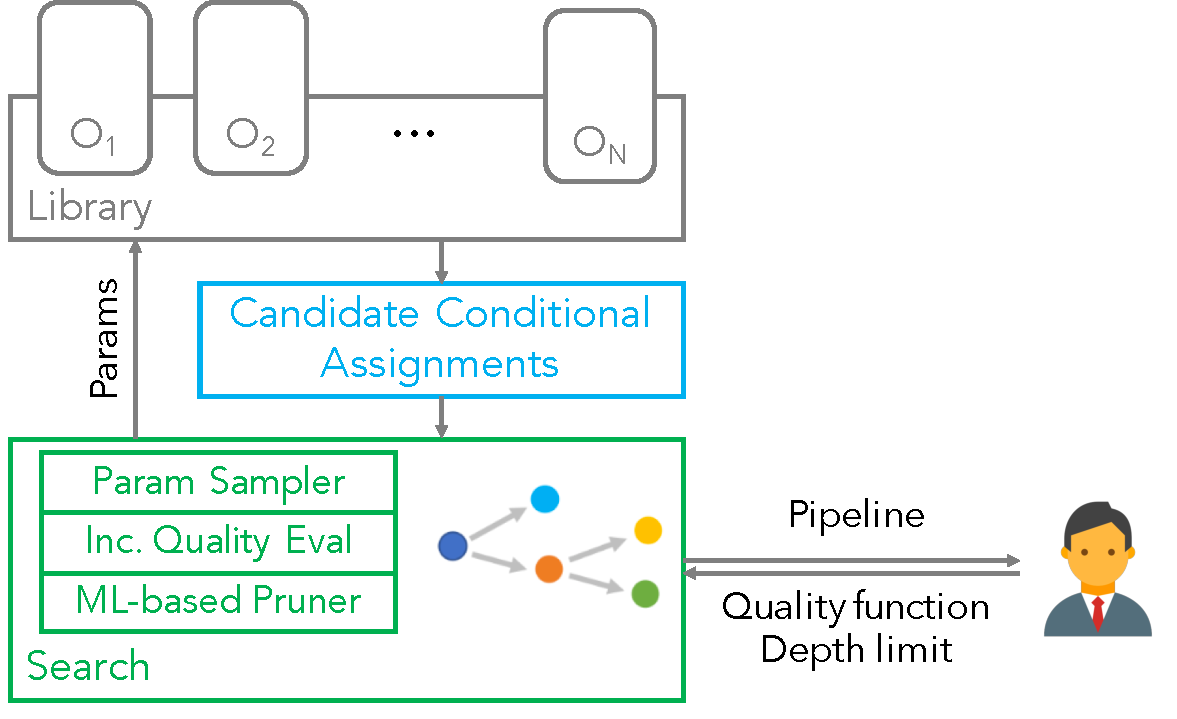
\includegraphics[width=0.7\columnwidth]{figures/arch}
 \caption{\small \sys decouples sampling from the parameter space from search. This allows the user to iterate quickly by observing early best-effort results. \label{fig:arch}}
\end{figure}



\section{Approach Outline}

\sys takes as input a user-provided quality function $Q$, and searches through the space of candidate pipelines $\mathcal{P}$ to find a cleaning pipeline $p*\in\mathcal{P}$ that maximizes the resulting quality of the relation $Q(p*(R))$.  \sys is progressive: at any time, \sys reports the best cleaning pipeline found so far.  This helps the user trade-off between search time and cleaning quality.  This section provides an architectural overview, and the subsequent section dive deeper into the implementation of the search algorithm and learning-based search-space pruning.

% Each conditional assignment can be appended to the current pool of candidate pipelines,  and then extend the current pool of candidate pipelines with the new condi  Thus the cost to execute a given cleaning operator can be an enormous bottleneck on the ability to generate candidate pipelines.  

%The space of possible conditional assignments and cleaning pipelines is far too large, and only a small subset is feasible to materialize at any time. 



\subsection{Synchronous Tuning}

Recall that a pipeline is composed of conditional assignments, which are generated by executing cleaning operators with specific parameter values.   A naive approach would select an operator $o$, draw a sample $\phi$ from its parameter space, execute $o(\phi)$ to generate a set of conditional assignments.      It then composes each conditional assignment $ca_i$ to each pipeline $p_j$ in the current pool of candidates, executes the new pipeline $p' = ca_i \circ p$, and evaluates the quality function $Q(p'(R))$.

Blackbox search algorithms typically couple the candidate (condition assignment) generation step with the quality evaluation step, because the former is usually very fast whereas quality evaluation may be slow.  In our context, the opposite is true, and quality evaluation is much faster than candidate generation.   Thus, the naive approach is susceptible to blocking on straggler cleaning operators that take a lon time to generate conditional assignments. 

\subsection{Asynchronous Architecture}

We propose a generate-then-search framework, that decouples the execution of cleaning operators and pipeline quality evaluation (Figure~\ref{fig:arch}).  A primary search process samples from each operator's parameter space and executes operators.  Each operator is run in a separate process and asynchronously adds to a shared pool of conditional assignments.  The search process manages the pool and draws from the pool to build data cleaing pipelines.  

One benefit of this asynchronous approach is that the search process does not block on a straggler cleaning operator.  It is common that operator parameters affect their runtime.  For example, inference thresholds and partitioning parameters can have ``cliffs'', where a small change in parameters can drastically slow down the performance of the method. Including such parameter settings in the search process naively would block the entire system.  In contrast, \sys will simply sample from faster operators until the slow inference task completes.  

One drawback of the asychronous approach is that the number of quality function evaluations is much higher\ewu{WHY?}. We argue that this is acceptable in many data cleaning settings, since quality function evaluation is often far cheaper than candidate repair generation (e.g., checking integrity constraints is cheaper than enforcing them). Furthermore, 


Our implementation simply allocates one process per operator, however this approach explicitly highlights the connection between the search space that is explored and resource scheduling.  For instance, allocating more CPU resources to slower cleaning operators would lead to a more uniform exploration of the search space.  We defer such investigation to future work.



% Our main architectural insight is a generate-then-search framework.  Possible parameter values are fed into a library of data cleaning methods, and these parameter assignments asynchronously generate candidate repairs to the dataset (called conditional assignments).  In parallel, a search thread builds a data cleaning plan using compositions of those transformations in the set.  Existing search algorithms implicitly pipeline these two steps; whereas, we decouple these two steps where candidate repairs can be generated in a separate thread and the search algorithm can proceed independently.  This contrasts from the baseline architecture, hereafter called \emph{synchronous tuning}, where a hyperparameter tuning algorithm will then select and assign parameter values to a sequence of operators and evaluate the quality at the end.  There are a few benefits for the asynchronous architecture of \sys.


% \vspace{0.5em} \noindent \textbf{Benefit 2. Progressive Results: } Next, the decoupling also allows for improved progressive behavior with early results. The search thread continuously polls the candidate conditional assignment set for new expansions. The naturally faster  data cleaning methods (e.g., approximate) will generate candidate repairs faster. Slower methods will eventually add these candidate repairs. This allows users to identify faults or glitches in their quality specifications or parameter spaces more quickly than if all methods were synchronously tuned in a pipeline.

\subsubsection{Parameter Space}
By default, users simply specify a list of allowable values for each operator parameter, and \sys samples from their values.  In addition, users can specify two types of parameters, for which \sys can apply search optimizations:

\begin{itemize}[leftmargin=*,topsep=.3em,itemsep=-.2em,partopsep=-.5em]
  \item \stitle{Attribute Name Parameters} If the parameter represents an attribute in the database, then \sys can infer the domain of allowable values.   For example, a numerical outlier detection algorithm might apply to a single attribute or a subset of attributes. \sys can also prune the paramater space by pruning attribute names that are irrelevant to the quality function.  

  \item \stitle{Threshold Parameters} Numeric parameters are often used as thresholds, inference parameters, or confidence bounds.  For these, users specify the most and least restrictive ends of the value domain, and \sys will sweep the space from most to least restrictive.   For instance, \texttt{ispell} only uses the dictionary if the attribute value is within \texttt{rec} characters of the dictionary word.  Thus, \sys will initially sample $\texttt{rec}=0$ and gradually relax the threshold.   
\end{itemize}

%which have the property that if the quality function    Another broad class of parameters in data cleaning methods are numerical parameters like thresholds and inference parameters. For these parameters, the user specifies a range (or a multi-dimensional grid). Often times, these parameters correspond to confidence metrics. In the example with the \texttt{City} table, the \texttt{ispell} method has a acceptance threshold for spell-checking. In these cases, we recommend that this search space is ordered fine-to-coarse. Where the most restrictive threshold is evaluated first towards increasingly less restrictive thresholds. 


\subsubsection{Incremental Quality Evaluation}

Most cleaning operators modify significantly fewer records than the entire dataset.  Since quality functions are simply aggregation queries, \sys can incrementally evaluate the quality function over the fixed records rather than the full dataset.  
This is exactly the process of incremental view maintenance, and we use standard techniques to incrementally compute quality functions that \ewu{HAVE X and Y properties}.  

Suppose we have relation $R$, quality function $q$, and a set of conditional assignment expressions $C$.  When possible, \sys computes $q(R)$ once and then for each of the expressions $c \in C$ compute a delta such $q(c(R)) = q(R) + \delta_c(q(R))$.
For many types of quality functions such incremental computation can be automatically synthesized and can greatly save on computation time.

Let us consider a concrete example with the quality function $q_1$, a functional dependency checker, from the previous section.
$R'$ is the resulting relation after applying \texttt{c} to all of the records.
Let $r_{pred}$ be the set of records that satisfy the predicate of the conditional assignment expression and $r_{pred}'$ be the resulting transformed records.
$q_1$ can be expressed in relational algebra in the following way:
\[
q_1(R') = \textsf{count}( R' \bowtie R' )
\]
$R'$ can be described in terms of $R$:
\[
R' = R - r_{pred} + r_{pred}' 
\]
leading to the following expression:
\[
q_1(R') = \red{q_1(R)} - \textsf{count}( r_{pred} \bowtie R )  + \textsf{count}( r'_{pred} \bowtie R )
\]
If we used a hash join to evaluate this quality function, the cost of incrementally maintaining is roughly linear in the size of the number records changed rather than the size of the relation.

% The consequence is that evaluating changes in quality can be very efficient for a large class of data cleaning problems.  The architecture of \sys is designed to exploit this property.  We assume conditional assignment generation to be expensive but quality evaluation to be fast.  An architecture that runs the entire pipeline before seeing the resultant quality is wasteful.



